\subsection{Metaheur\'istica ACO}
\begin{frame}{Hormigas}
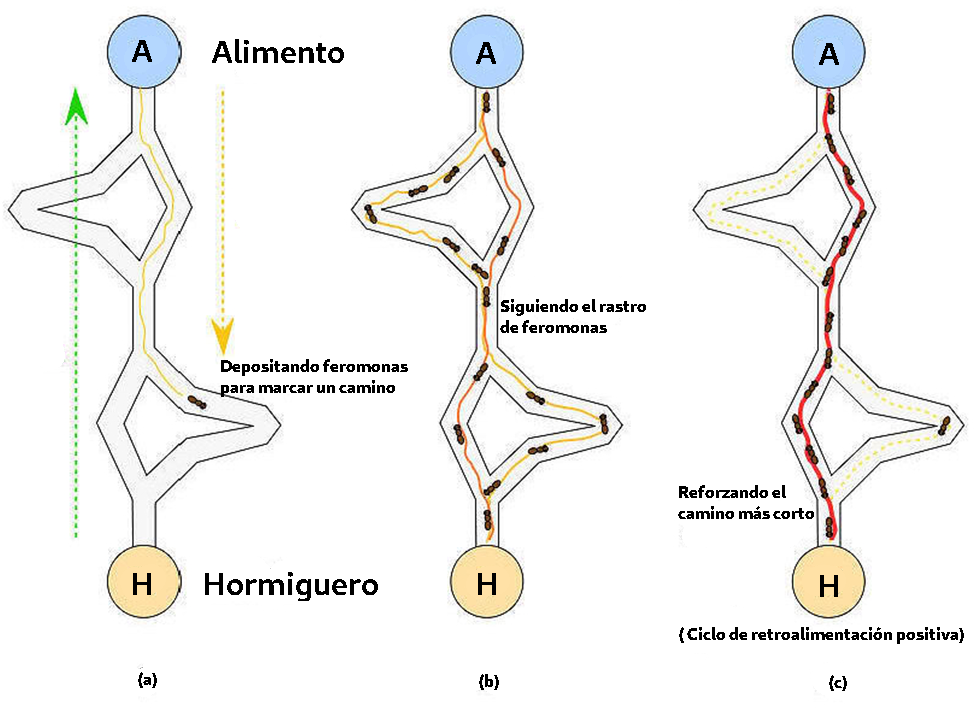
\includegraphics[width=0.9\textwidth]{Pictures/ACO-ant.png}
\end{frame}

\begin{frame}{Hormigas}
\centering
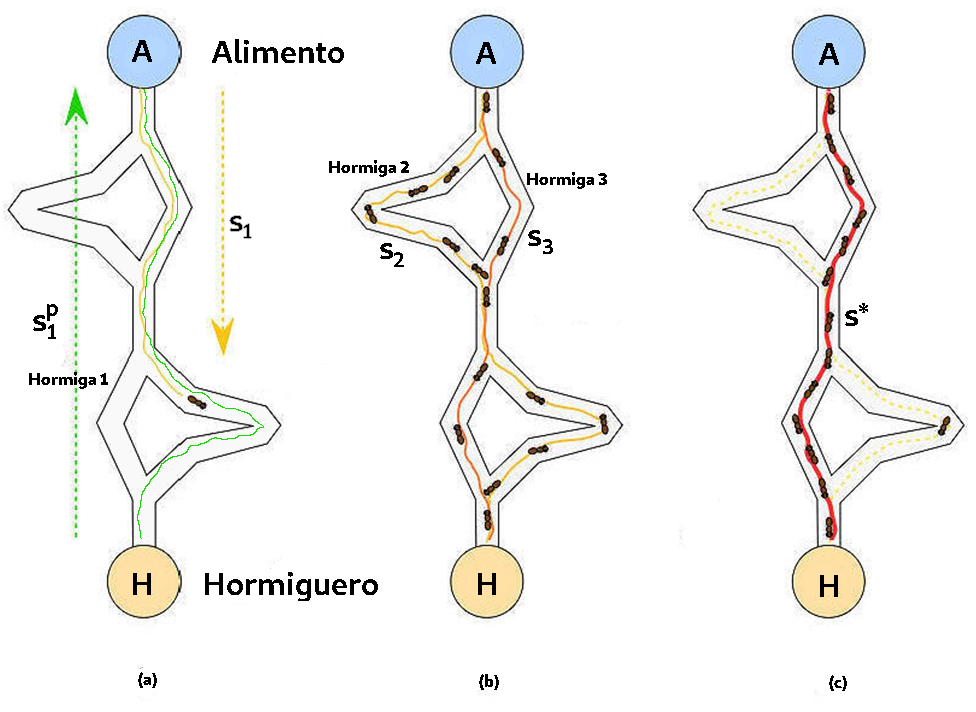
\includegraphics[width=0.9\textwidth]{Pictures/ACO-ant-2.png}
\end{frame}

\begin{frame}{Modelo de Feromonas}
\begin{itemize}
    \item Comunicaci\'on indirecta mediante feromonas
    \item Recorrido aleatorio
    \item Convergencia sobre el camino m\'as corto
\end{itemize}
    \begin{algorithm}[H]
    \SetAlgoLined
     Ajuste de Par\'ametros \& inicializaci\'on de feromonas\;
     \While{Criterio de finalizaci\'on no se cumple}{
       Construcci\'on\_de\_soluci\'on\_de\_cada\_hormiga()\;
       M\'etodo\_de\_b\'usqueda\_no\_local(); //Paso opcional\\
       Actualizaci\'on\_de\_feromonas()\;
     }
     \caption{Algoritmo metaheur\'istica ACO}\label{ACO-Algo}
    \end{algorithm}
\end{frame}

\begin{frame}{Adaptaci\'on de ACO a un problema de satisfacci\'on de restricciones}
    \begin{itemize}
        \item Hormigas Sint\'eticas o Agentes
        %\item Basado en el comportamiento de las hormigas reales
        \item Entendiendo los caminos posibles a recorrer por las hormigas como un grafo
        \item Camino $s$ compuesto por aristas o componentes de soluci\'on $c_i$
        \item Valor de la feromona depositada $\tau_{i}$
        \item Se pueden agregar restricciones $\Omega$ en el desplazamiento
    \end{itemize}
\end{frame}

\subsection{Problema de Satisfacci\'on de Restricciones}
\begin{frame}{ACO aplicado como Problema de Satisfacci\'on de Restricciones}
  \begin{columns}
    \begin{column}{0.5\textwidth}
        \begin{itemize}
          \item $P = (S, \Omega, F)$
          % esta definido por un conjunto discreto de variables
          \item S:  Cjto. de soluciones, compuesto por variables discretas $X_{i}$, $i \in 1 \dotsc n$
          %\item $S:\quad X = v_{i}^{j} \in D_{i} = \{v_{i}^{1} \dotsc  v_{i}^{|D_{i}|}\}$.
          \item Sol. Candidata $s \in S$, y $s^{*}$ una soluci\'on \'optima
          \item Cjto. de Restricciones $\Omega$
          \item Funci\'on objetivo $F: S\rightarrow \mathbb R_{0}^{+}$
          %\item  
          
      \end{itemize}
    \end{column}
    \begin{column}{0.5\textwidth}
      \begin{itemize}
          \item $s$ es factible si satisface las restricciones de $\Omega$
          % y se relacionan mediante 
          \item Pueden existir m\'ultiples soluciones $s^{*}$
          \item $S^{*}$ es el conjunto que engloba todas las soluciones \'optimas
          \item $s^{*} \in S^{*} \subseteq S$
      \end{itemize}
    \end{column}
\end{columns}
\end{frame}


\begin{frame}{Individualizaci\'on de Filamentos como un Problema de Satisfacci\'on de Restricciones}
    \begin{itemize}
    \item Se desconoce a priori el n\'umero de filamentos a buscar.%, dado que una imagen puede tener individualizaciones distintas para 2 expertos.
    \item Generalmente se busca individualizar m\'as de un filamento por imagen, lo que conlleva a elegir los mejores filamentos entre las soluciones que se encuentren.
    \item El uso de un grafo para representar la red de filamentos puede implicar que las combinaciones de soluciones crezcan de manera exponencial.
\end{itemize}
\end{frame}


% \begin{frame}{Adaptaci\'on a Individualizaci\'on de Filamentos}
%     \begin{algorithm}[H]
%     \SetAlgoLined
%     \KwData{Variables $X_i \dotsc X_n$, dominios $D_1 \dotsc D_n$, Restricciones $\in \Omega$}
%     \KwResult{conjunto s\textquotesingle $ \subseteq S$ != $\emptyset$, si existen soluciones factibles}
%      Ajuste de Par\'ametros \& inicializaci\'on de feromonas \;
%      \While{Criterio de finalización no se cumple}{
%       Construcci\'on\_de\_soluci\'on\_de\_cada\_hormiga()\;
%       M\'etodo\_de\_b\'usqueda\_no\_local(); //Paso opcional\\
%       Actualizaci\'on\_de\_feromonas()\;
%      }
%      \caption{Algoritmo de un modelo COP adaptado a una metaheur\'istica ACO}\label{COP-ACO-Algo}
%     \end{algorithm}
% \end{frame}


\section{Algoritmo Propuesto}
\begin{frame}{ACO: Construcci\'on de Soluci\'on}
\centering
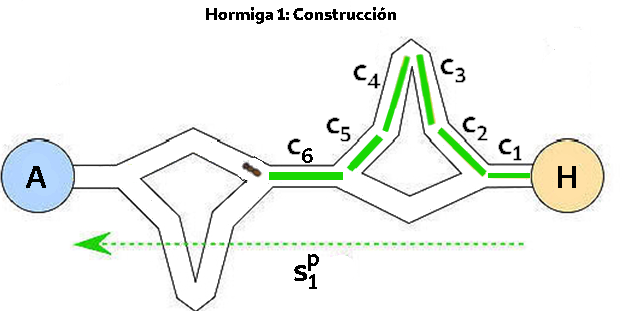
\includegraphics[scale=0.35]{Pictures/ACO-ant-Constr.png}
\begin{itemize}
    \item Elecci\'on de Aristas/Componentes $c_i$ que respeten restricciones en $\Omega$
    \begin{equation}
P(c_{ij} | s^{P}) = \frac
        {\tau_{ij}^{\alpha} ~ \eta_{ij}^{\beta}}
        {\sum\limits_{c_{ij}\in N(s^p)}{\tau_{ij}^{\alpha} ~ \eta_{ij}^{\beta} } }, \forall c_{ij} \in N(s^{P}).
\label{eq:antProbabilities}
\end{equation}
\end{itemize}
\end{frame}

\begin{frame}{ACO: Construcci\'on de Soluci\'on}
\centering
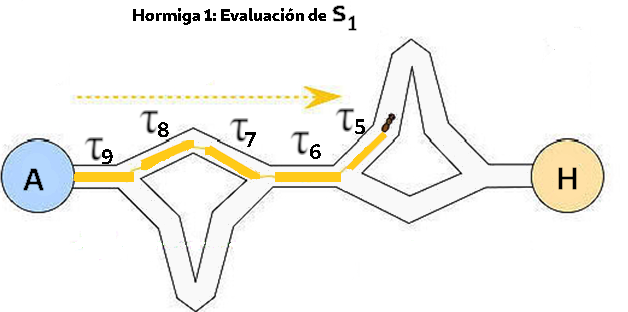
\includegraphics[scale=0.4]{Pictures/ACO-ant-ferom.png}
\begin{itemize}
    \item Evaluaci\'on de factiblidad de soluciones candidatas $s \in S$
\end{itemize}
\end{frame}





\subsection{Inicializaci\'on ACO}
\begin{frame}{Par\'ametros}
    \begin{itemize}
        \item 
    \end{itemize}
\end{frame}
\subsection{Construcci\'on de Soluciones}
\begin{frame}{Elecci\'on de Aristas $c_i$}

    
\end{frame}
\subsection{Anti-Feromonas}
\subsection{M\'etodo de b\'usqueda no local}